\chapter{Perspective}
\mytop{In this chapter we will look at some ways of improving the two implemented algorithms and the GUI, if the application should go from proof of concept to an finished application.}

\section{General Improvements}
Improving the application from a proof of concept to a finished application our GUI could be improved by making the cube in the application into 3D. Furthermore we could make our application multithreaded, this would give a lot of possibilities. 


\section{Improving the Algorithms}
The two algorithms can be improved in several ways. How this can be done will be described in the following.
In order to understand this section it is necessary to have read the general description of the beginner's algorithm and Kociemba's optimal solver (see chapter \ref{cha:solvingAlgorithms}) and the descriptions of our implementations (see chapter \ref{chap:beginnerImplement} and \ref{chap:kociembaImplement}).

\subsection{Beginner's Algorithm}
When describing the improvement of the beginner's algorithm, the improvements are described step by step. 
A twist sequence which leads to the next step may be the most efficient for doing just that, but can potentially cause the entire twist sequence from the scrambled state to the solved state to be longer. 
i.e. a long partial twist sequence may lead to a shorter overall twist sequence. In order to utilize this a lot of analysis is necessary, which is nearly impossible for a person to perform and would take a large amount of time to implement.
Additionally the algorithm still has to be the beginner's algorithm, which means that the steps used in the beginner's algorithm are also implemented and not just swapped for more efficient ones, which would defeat the purpose of implementing the beginner's algorithm.


The beginner's algorithm is as mentioned before a very twist-wise inefficient solving algorithm. 
There are however quite a few areas in which the implementation can be improved.
In the first step (see subsection \ref{sub:step1}) choosing the correct face to be the face of the first layer will decrease the number of twists needed to complete the first step, since a different part of the cross is assembled on the different faces.

In the second step (see subsection \ref{sub:step2}), where the corners needs to be positioned in the first layer, there are generally two ways to improve the algorithm.
The first way to improve the twist sequence in this part is to choose the most efficient order of positioning the corners.
Finding out which order is the most efficient one may seem to require a large amount of analysis, but since only four corners needs to be positioned a simulation can be used with advantage.
There are generally $4! = 4 \cdot 3 \cdot 2 \cdot 1 = 24$ possible orders the corners can be positioned in, which makes the process of computing the shortest twist sequence a rather simple task.
The other way to improve this step is to eliminate the repetition of an algorithm. 
The algorithm used for rotating a corner \cpiece{} in our implementation only rotates it in one direction. 
If an algorithm for rotating a corner \cpiece{} the other direction were implemented it would reduce the number of times the algorithms would be used.

In the third step (see subsection \ref{sub:step3}), where the edge \cpiece{}s are positioned in the second layer, there is only one way to improve it; choosing the most efficient order to position the edge \cpiece{}s. Since there are four edge \cpiece{}s that need to be positioned, the logic used in improving the second step can be applied in the third step.

In the fourth step (see subsection \ref{sub:step4}), where the last layer cross is fully attained, there is only room for little improvement, if the algorithm should still be the beginner's algorithm.
As mentioned in (see subsection \ref{sub:step4}), there are three possible settings of the unsolved cross.
In the position known as the opposite L, the reverse of the algorithm used in this step will skip the next setting and directly give the solved cross.
This can potentially reduce the solving algorithm by six twists.


The fifth and final step of the beginner's algorithm (see subsection \ref{sub:step5}) is divided into two methods in our implementation.


The first method of the final step, which positioned the remaining four corners correctly, only uses a single algorithm.
This algorithm rotates three corner \cpiece{}s' positions counterclockwise.
Half the time the corner \cpiece{}s' positions needs to be rotated clockwise, which means that this algorithm is used twice.
Its reverse can be used to rotate the corner \cpiece{}s' positions clockwise, which will in those cases when needed reduce the solving twist sequence by eight.

When using the half turn metric the second method of the final step cannot be improved while staying true to our description of the beginner's algorithm (see section \ref{sec:beginner}).
\subsection{Kociemba's Optimal Solver}
When we look at improving our implementation of Kociemba's optimal solver some different things can be done.
	
In the first phase of our implementation of Kociemba's optimal solver it checks after every tested move sequence if the \cube{} is in \m{H}.
This \m{H} is with respect to the primary \face{}s (see subsection \ref{sub:theSubgroupH}), but it is also possible for the \rubik{} to be inside \m{H} with respect to the secondary or tertiary \face{}s, see figure \ref{fig:secondaryH}.

\begin{figure}[htb]
	\centering
	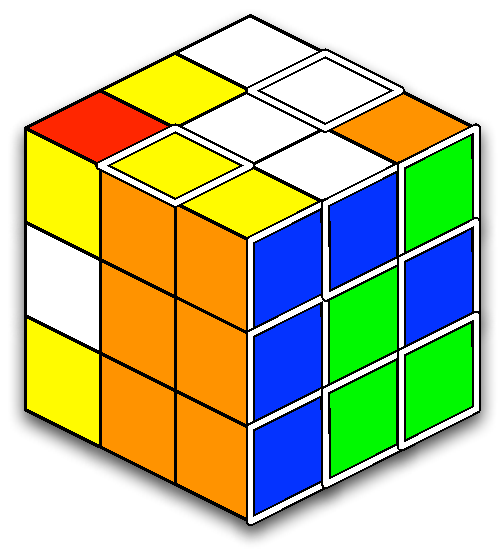
\includegraphics[scale=0.75]{input/pics/secondaryH.pdf}
	\caption{\myCaption{A scrambled Rubik's Cube which is inside secondary \m{H}, but not primary.}}
	\label{fig:secondaryH}
\end{figure}

As with primary \m{H}, the secondary \m{H} must meet the specifications:
Every secondary \facelet{} must be on the secondary \face{}s, and the edges not in a secondary \face{} must be orientated correctly.
These specifications are seen to be met in figure \ref{fig:secondaryH}.

\begin{comment}
When the \rubik{} is solved from an arbitrary position into H it is not possible to look at it from other angels. 
This means that the application will always work with the \face{}s turning the same way (see subsection \ref{sub:cubeFaces}).
To improve this the \rubik{} could be turned around shifting the \face{}s in the application.
This means that instead of testing if the primary \face{} \cubie{}s are orientated correct it would test if the secondary \face{} \cubie{}s are orientated correct. 
The same idea also applies to the tertiary \face{}.
\end{comment}
	
To decrease the search time when solving a \rubik{}, every know position of the \rubik{} could be saved in a look up table.
When a shortest path to that position is found it could be saved.
This would shorten the time to solve the \rubik{} if the position is already know.
If this is combined with the previous improvement suggestion it could make the search time to get into \m{H} shorter.
Turning of the \face{}s only apply outside \m{H} since it would have a negative effect inside \m{H}. 
	 
The program is built up around one \cube{} object.
As a result of this the computer is only able to use one CPU core to work on that \cube{}.
With some modifications it could be possible make a copy of this \cube{} object.
This will make it possible to work on more than one \cube{} object with the same starting position.
It would be possible to make the application multithreaded in alot of ways.
When the application is working outside \m{H} it is working with \m{S} moves.
Here it is possible to make a new thread for every depth the method searches in.
In the same way it is possible to make a new thread for every search depth inside \m{H}.
But there are still more ways to improve the algorithm with multithreading.
The last way we will mention is when searching in general the moves in \m{S} and \m{A} could be divide and a new thread could be made for these new groups of moves.

\mytail{As stated in this chapter there is still room for improvements if we were to finish the application.}